\documentclass[a4paper,12pt]{article} 


\usepackage[T2A]{fontenc}			
\usepackage[utf8]{inputenc}			
\usepackage[english,russian]{babel}	

\usepackage{graphicx, scalerel}    
\usepackage{wrapfig}               
\usepackage[14pt]{extsizes}        
\usepackage[warn]{mathtext}       
\usepackage{indentfirst}      
\usepackage[margin = 25mm]{geometry}
\usepackage[table,xcdraw]{xcolor} 
\usepackage{amsmath,amsfonts,amssymb,amsthm,mathtools}
\usepackage{wasysym}                
\usepackage{upgreek}                
\usepackage{caption}
\usepackage{multirow}
\captionsetup{labelsep=period}
\usepackage[font=small,labelfont=bf]{caption}
\usepackage{gensymb}
\usepackage[unicode, pdftex]{hyperref}
\usepackage{tikz}
\usetikzlibrary{positioning}
\usepackage{fancyhdr}
\pagestyle{fancy}
\setlength\fboxsep{3pt} % Отступ рамки \fbox{} от рисунка
\setlength\fboxrule{1pt} % Толщина линий рамки \fbox{}
\newcommand{\tocsection}[1]{\section*{#1} \addcontentsline{toc}{section}{#1}}
\newcommand{\tocsubsection}[1]{\subsection*{#1} \addcontentsline{toc}{subsection}{#1}}
\renewcommand{\cftsecleader}{\cftdotfill{\cftdotsep}}

\def\fillandplacepagenumber{%
	\par\pagestyle{empty}%
	\vbox to 0pt{\vss}\vfill
	\vbox to 0pt{\baselineskip0pt
		\hbox to\linewidth{\hss}%
		\baselineskip\footskip
		\hbox to\linewidth{%
			\hfil\thepage\hfil}\vss}}

\begin{document}
		\newcommand{\HRule}{\rule{\linewidth}{0.7mm}} % Defines a new command for the horizontal lines, change thickness here

\begin{center}
	\large\textbf{Московский Физико-Технический Институт}\\
	\large\textbf{(государственный университет)}
	
	\vfill
	

	
	\Large Вычислительная математика
	%----------------------------------------------------------------------------------------
	%	TITLE SECTION
	%----------------------------------------------------------------------------------------
	
	\HRule
	\\[0.4cm]
	{ \huge \bfseries Лабораторная работа №9}
	\\[0.4cm] % Title of your document
	\HRule
	\\[0.5cm]
	
	\ \\
	\textbf{\large Автор:} \\	
	\large Овсянников Михаил Б01-008\\
	\vfill
	\hspace*{-0.8 cm}
\includegraphics[width=100 pt]{./Include/frkt_logo.pdf}\\
	\large Долгопрудный, 2023
\end{center}

\thispagestyle{empty}

\newpage
\setcounter{page}{2}
\fancyfoot[c]{\thepage}
\fancyhead[L] {Лабораторная работа №9}
\fancyhead[R]{}

		\tableofcontents
		\newpage
		
		\tocsection{Цель}
		Реализовать метод стрельбы для решения краевых задач.
			
		\tocsection{Теоретические сведения}
		\tocsubsection{Общая задача}

		У нас есть какое-то дифференциальное уравнение:
		\begin{equation*}
			y'' = f(x, y, y')
		\end{equation*}
		
		И пускай вдобавок на решение наложено какое-то условие $F(y, y', y'') = 0$, которое может быть как алгебраическим уравнением, связывающим соответствующие переменные, так и полноценным функционалом над ними.
		
		
		Требуется отыскать решение, удовлетворяющее самому уравнению и дополнительно поставленному условию. 
		
		На помощь приходит так называемый метод стрельбы, который и реализован в данной работе.
		
		
		\tocsubsection{Описание метода стрельбы}

		Построение метода стрельбы начинается с введения в нашу задачу дополнительного параметра $\alpha$. Допустим, если дополнительное условие $F$ позволяет, следующим образом:
		\begin{equation*}
			y'(a) = \alpha,
		\end{equation*}
	
		\noindent где $a$ -- левый конец отрезка интегрирования уравнения.
		
		Если теперь мы решим поставленную задачу Коши при конкретном $\alpha$, то мы получим какую-то функцию $y^0(x)$, которая скорее всего не будет удовлетворять условию $F(y, y', y'') = 0$. Однако мы можем проделать все то же самое и при других значениях $\alpha$. Таким образом, мы получим зависимость $F(\alpha)$. И всё, что нам теперь нужно, -- это решить уравнение $F(\alpha) = 0$. Это можно сделать методом Ньютона:
		\begin{equation*}
			\alpha^{n+1} = \alpha^n - \frac{F(\alpha^n)}{F'(\alpha^n)}.
		\end{equation*}
	
		Но что же такое $F(\alpha^n)$ в данном случае? И как его посчитать? С этими вопросами дело обстоит хуже -- это специфично для задачи. Рассмотрим лишь подход, наводящий на мысли, как посчитать эту величину.
		
		Мы имеем дело с системой:
		\begin{equation*}
			\begin{cases}
				y'' = f(x, y, y'), \\
				y(0) = y_0, \\
				y'(0) = \alpha.
			\end{cases}
		\end{equation*}
	
		Сначала преобразуем уравнение 2-ой степени в систему из двух уравнений 1-ой степени заменой $y = y$, $y' = u$:
		\begin{equation}
			\begin{cases}
				y' = u, \\
				u' = f(x, y, u), \\
				y(0) = y_0, \\
				u(0) = \alpha.
			\end{cases}
		\end{equation}
	
		В нашей задаче считаем $y$ дважды непрерывно дифференцируемой, поэтому без зазрения совести продифференцируем последнюю систему по параметру $\alpha$. Обозначим $A = \frac{\partial y}{\partial \alpha}$, $B = \frac{\partial u}{\partial \alpha}$. Тогда:
		\begin{equation}
			\begin{cases}
				\frac{dA}{dx} = B, \\
				\frac{dB}{dx} = \frac{\partial f}{\partial y} A + \frac{\partial f}{\partial u} B, \\
				A(0) = 0, \\
				B(0) = 1.
			\end{cases}
			\label{AB_SYS}
		\end{equation}
	
		Тогда:
		\begin{equation*}
			F'(\alpha) = \frac{\partial F}{\partial y} \cdot \frac{\partial y}{\partial \alpha} + 
			\frac{\partial F}{\partial y'} \cdot \frac{\partial y'}{\partial \alpha} + 
			\frac{\partial F}{\partial y''} \cdot \frac{\partial y''}{\partial \alpha} 
		\end{equation*}
	
		Соответствующие производные найдем как:
		\begin{itemize}
			\item $\frac{\partial y}{\partial \alpha} = A$
			
			\item $\frac{\partial y'}{\partial \alpha} = B$
			
			\item $\frac{\partial y''}{\partial \alpha} = \frac{\partial f}{\partial y} \cdot \frac{\partial y}{\partial \alpha} + \frac{\partial f}{\partial y'} \cdot \frac{\partial y'}{\partial \alpha} =
		    A\frac{\partial f}{\partial y} + B\frac{\partial f}{\partial y'}$.
		\end{itemize}
	
		Отсюда и начинаем итерировать, используя метод Ньютона. На каждом шаге мы получаем не просто значение, а целую функцию!
		
		Перейдем непосредственно к поставленной задаче.

		
		\tocsection{Данная задача}
		\tocsubsection{Постановка задачи}
		В качестве примера был выбран номер \textbf{XI.9.3} второй части сборника Аристовой и Лобанова:
		\begin{equation*}
			\begin{cases*}
				y'' - x\sqrt{y} = 0, \;\;\;\;\;\;\; 0 \leqslant x \leqslant 1, \\
				y(0) = 0, \\
				\displaystyle\int\limits_{0}^{1} y(x)dx = 1.
			\end{cases*}
		\end{equation*}
	
		Введем в качестве параметра начальное условие на производную -- $y'(0) = \alpha$. Тогда полученная задача отлично подходит под заготовленный выше шаблон.
	
		Поскольку метод стрельбы заключает в себе некую специфичность в определении $F'(\alpha)$, найдем эту величину конкретно для этой задачи:
		\begin{equation*}
			F(\alpha) = -1 + \displaystyle\int\limits_{0}^{1} y(x)dx.
		\end{equation*}
	
		Тогда:
		\begin{equation*}
			F'(\alpha) = \frac{d}{d\alpha}\displaystyle\int\limits_{0}^{1} y(x)dx = \displaystyle\int\limits_{0}^{1} \frac{\partial y}{\partial \alpha}(x) dx = \displaystyle\int\limits_{0}^{1} A(x) dx.
		\end{equation*}
	
		Сама же система \eqref{AB_SYS} принимает вид:
		\begin{equation*}
			\begin{cases}
				\frac{dA}{dx} = B, \\
				\frac{dB}{dx} = \frac{x}{2\sqrt{y}} A, \\
				A(0) = 0, \\
				B(0) = 1.
			\end{cases}
		\end{equation*}
	
		В имеющейся реализации эти системы решаются одновременно и сразу же с этим всем считаются интегралы для $F(\alpha)$ и $F'(\alpha)$.
	
	
		\newpage
		\tocsubsection{Результаты}

		Поскольку используется метод Ньютона, то решение находится быстро. Представим график решения:

		\begin{figure}[h!]
			\centering
			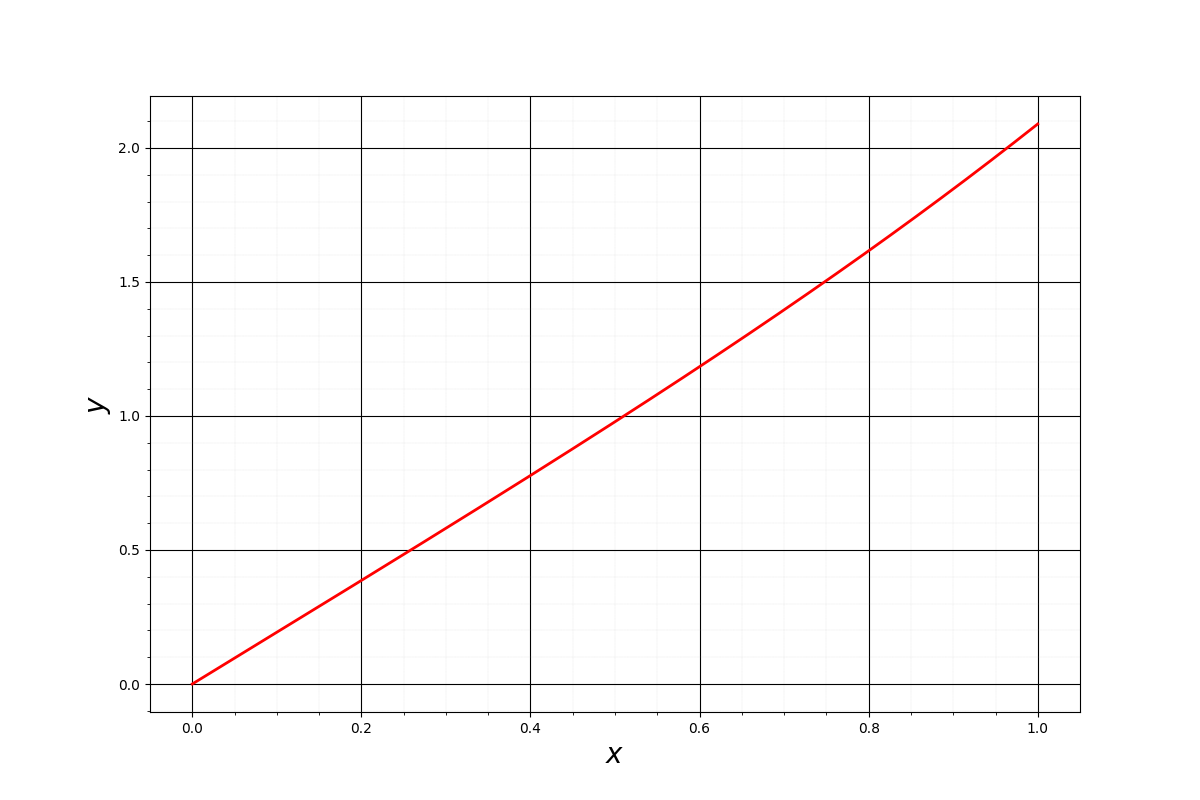
\includegraphics[width=0.95\linewidth]{Pictures/Plot.png}
			\caption{Решение системы при условии $F(y, y', y'') = 0$}
		\end{figure}
	
		Оно чрезвычайно сильно похоже на прямую -- но это не так.
		
		Значение $\alpha$, при котором нашлось решение: $\;\; 1.9291176846202034$. 
		
		Само же значение интеграла получилось $     I = 0.9999999999919321$.
	
	
	
	
		
		\tocsection{Вывод}
		В работе был изучен и реализован метод стрельбы для решения краевой задачи. Он сходится достаточно быстро, а решение получается приемлемо точным.
		
		
\end{document}